%!TeX spellcheck = de_DE

\input{00_common/common_head.tex}
\newcommand\Warning{%
 \makebox[1.4em][c]{%
 \makebox[0pt][c]{\raisebox{.1em}{\small!}}%
 \makebox[0pt][c]{\color{red}\Large$\bigtriangleup$}}}%

\title{Übung zum\linebreak[1]C/C++-Praktikum\linebreak[1] Fachgebiet Echtzeitsysteme \linebreak[1]\linebreak[1] (Embedded) C}

\setcounter{section}{19}

%optional parameters to speed up build (increases pdf file size)
%\pdfcompresslevel=0
%\pdfobjcompresslevel=0
\begin{document}

\maketitle

\setcounter{tocdepth}{1}
\setlength\cftsecnumwidth{10em}
\setlength\cftbeforesecskip{.1em} % line skip between sections ("sec")

\setHeader{Aufgaben zu Embedded C}

\input{05_c/problems/cIntro}
\optionaltextboxInternal{%
\Warning \; Die folgendenden Aufgaben sind nur zur Bearbeitung mit dem ausleihbaren Evaluationsboard gedacht. \Warning}
\input{05_c/problems/mcIntro}
\input{05_c/problems/mcButton}
\input{05_c/problems/mcDisplay}
\input{05_c/problems/mcJoysticks}
\input{05_c/problems/mcTouchScreen}
\input{05_c/problems/mcGame}
% !TeX spellcheck = de_DE
\section{\ExercisePrefixEmbeddedC DHT11 \optional}

\optionaltextbox

Für die folgende Aufgabe musst du dir folgendes zusätzliches Material bei den Betreuern beschaffen:
\begin{itemize}
\item DHT11 Temperatur- und Feuchtigkeitssensor
\item 3 Steckbrücken Pin-Pin 20cm (jeweils ein verbundenes Steckbrückenpaar und eine einzelne Steckbrücke)
\item 1 Steckbrücke Pin-Buchse 20cm
\item 1 Widerstand \SI{10}{\kilo\ohm} (oder höher)
\end{itemize}

Der DHT11 ist ein Temperatur- und Feuchtigkeitssensor, der mithilfe des Steckplatine an den Microcontroller angeschlossen werden kann.
Der DHT11 hat 4 Anschlüsse (Pins), von denen im Rahmen des Praktikums 3 verwendet werden.
Zwei Pins werden für Masse (\lstinline|GND|) und Versorgungsspannung (\lstinline|VCC|) genutzt und ein Pin für die digitale Datenübertragung zwischen dem DHT11 und dem Microcontroller.
Abbildung \ref{fig:dht11Pins} zeigt die Pin-Belegung des DHT11.
Pin 1 wird mit \lstinline|VCC| verbunden und Pin 4 mit \lstinline|GND|.
Pin 2 ist ein I/O-Pin zur digitalen Datenübertragung.
In dieser Aufgabe ist es das Ziel die Temperatur- und Feuchtigkeitswerte des Sensors kontinuierlich auszulesen und diese auf dem Display darzustellen.
\begin{figure}[!htb]
	\centering
	\includegraphics[width=0.2\textwidth]{./05_c/figures/DHT11.png}
	\caption{DHT11 Pinbelegung}
	\label{fig:dht11Pins}
\end{figure} 

\begin{enumerate}
\item 
Zunächst trenne den Microcontroller von der Stromzufuhr und stelle sicher, dass dieser ausgeschaltet ist.
Verbinde gemäß Abbildung \ref{fig:dht11Schematics} den DHT11 mit dem Microcontroller.
Der DHT11 wird, von links gezählt, an den dritten Pin des CN17 Steckers des Microcontrollers angeschlossen (Port 5, Pin 2, Präprozessorkonstante \lstinline|GPIO1PIN_PF52|).
Nutze als Unterstützung Abbildung~\ref{fig:cpppWiring}, die schematisch die GPIO-Verbindungen des Microcontrollers darstellt.
Bevor der Microcontroller wieder an den Computer angeschlossen wird, lasse die Verkabelung von einem Tutor überprüfen.
%
\begin{figure}[!htb]
	\centering
	\includegraphics[width=0.35\textwidth]{./05_c/figures/DHT11-Schematics.pdf}
	\caption{Verkabelung des DHT11}
	\label{fig:dht11Schematics}
\end{figure} 
\begin{figure}[!htb]
	\centering
	\includegraphics[width=0.7\textwidth]{./05_c/figures/cppp-wiring.pdf}
	\caption{Verkabelung des DHT11}
	\label{fig:cpppWiring}
\end{figure} 

\item 
In der Funktion \lstinline|readDHT11(uint8_t* humidity, uint8_t* temperature)| in der Datei \filename{dht11.c} wird zunächst eine Präambel vom DHT11 an den Microcontroller gesendet.
Hierdurch wird die Verbindung zwischen dem DHT11 und dem Microcontroller synchronisiert. 
Nach der Präambel beginnt der DHT11 40 Bits an den Microcontroller zu senden.
Abbildung \ref{fig:dht11Package} zeigt die Aufteilung der Bitgruppen.

Implementiere die fehlenden Stellen der Funktion \lstinline|readDHT11(uint8_t* humidity, uint8_t* temperature)|, indem du folgende Teilschritte umsetzt.
Nach der Präambel müssen zunächst die ankommenden Signale als 40~Bits interpretiert und in einem Array mit 5~Einträgen je 8~Bits gespeichert werden.
Lese mit \lstinline|Gpio1pin_Get(GPIO1PIN_P52)| den aktuellen Wert des digitalen Pins aus und entscheide entsprechend der folgenden Logik, ob es sich um eine 1 oder 0 handelt.
Ist der Pin länger als \SI{30}{\micro\second} auf \lstinline|HIGH| gesetzt $t_{HIGH} > \SI{30}{\micro\second}$, dann interpretiere dieses Signal als eine 1 und im umgekehrten Fall $t_{HIGH} < \SI{30}{\micro\second}$ als eine 0.
Nachdem alle 40 Bits empfangen wurden, bilde die Checksumme, welche die Summe der ersten 32 Bits darstellt. 
Ist der folgende Pseudocode erfüllt, dann ist die Übertragung der Daten erfolgreich gewesen.
%
\cpppInputListing{05_c/listings/dht11_checksum.c}
%
Beende die Methode  \lstinline|readDHT11readDHT11|, sofern die Checksumme nicht stimmt. 
Ist die Checksumme richtig, speichere die aktuelle Temperatur und Feuchtigkeit in den übergebenen Parametern \lstinline|humidity| und \lstinline|temperature|.
\begin{figure}[!htb]
	\centering
	\includegraphics[width=0.7\textwidth]{./05_c/figures/dht11Bits.pdf}
	\caption{40 Bit Datenstruktur eines DHT11 Pakets}
	\label{fig:dht11Package}
\end{figure} 
\hints{
	\item Bei der Abfrage des Pins mithilfe von \lstinline|Gpio1pin_Get(GPIO1PIN_P52)|, kann es dazu kommen, dass fehlerhafte Signale dauerhaft auf \lstinline|HIGH| oder \lstinline|LOW| bleiben.
	Um diesen Fall zu filtern, verwende folgende Art der Abfrage.
	\cpppInputListing{05_c/listings/dht11.c}
	
	\item Um einen Delay auf dem Microcontroller ausführen, kannst du die Methode \lstinline|microDelay(uint32_t timeInMicroseconds)| verwenden. Zum Beispiel wird beim Aufruf  \lstinline|microDelay(20)| der Microcontroller \SI{20}{\micro\second} pausiert.
	
	\item Der DHT11 sendet immer seine Daten geordnet nach dem höchsten Bit, sodass der höchstwertigste Bit zuerst gesendet wird.
}

\item 
Nutze die Methoden \lstinline|writeTextln| und \lstinline|writeNumberOnDisplay| der Display-Library, um die Sensorenwerte auf dem Display auszugeben.

\hints{
	\item 
	Falls du die Funktionen \lstinline|writeTextln| und \lstinline|writeNumberOnDisplay| noch nicht implementiert hast, kannst du die Methoden der Musterlösung mit der Konkatenation des Suffix \lstinline|_s| nutzen (also bspw. \lstinline|writeTextln_s| und \lstinline|writeNumberOnDisplay_s|).
}

\end{enumerate}
\section{\ExercisePrefixEmbeddedC Beschleunigungssensor \optional}

Auf der Platine des FM4 Mikrocontrollers ist ein Beschleunigungssensor eingebaut, den du verwenden kannst um die Orientierung des Entwicklungsboards auszulesen. In der Library des Templates wird dir die Schnittstelle \lstinline|acceleration_app.h| zur Verfügung gestellt mit der du den Beschleunigungssensor für eine eigene Applikation verwenden kannst. In dieser Aufgabe wirst du ein Programm schreiben, mit dem du den Beschleunigungssensor nutzen kannst um eine digitale Wasserwaage zu simulieren. 
\begin{figure}[!htb]
	\centering
	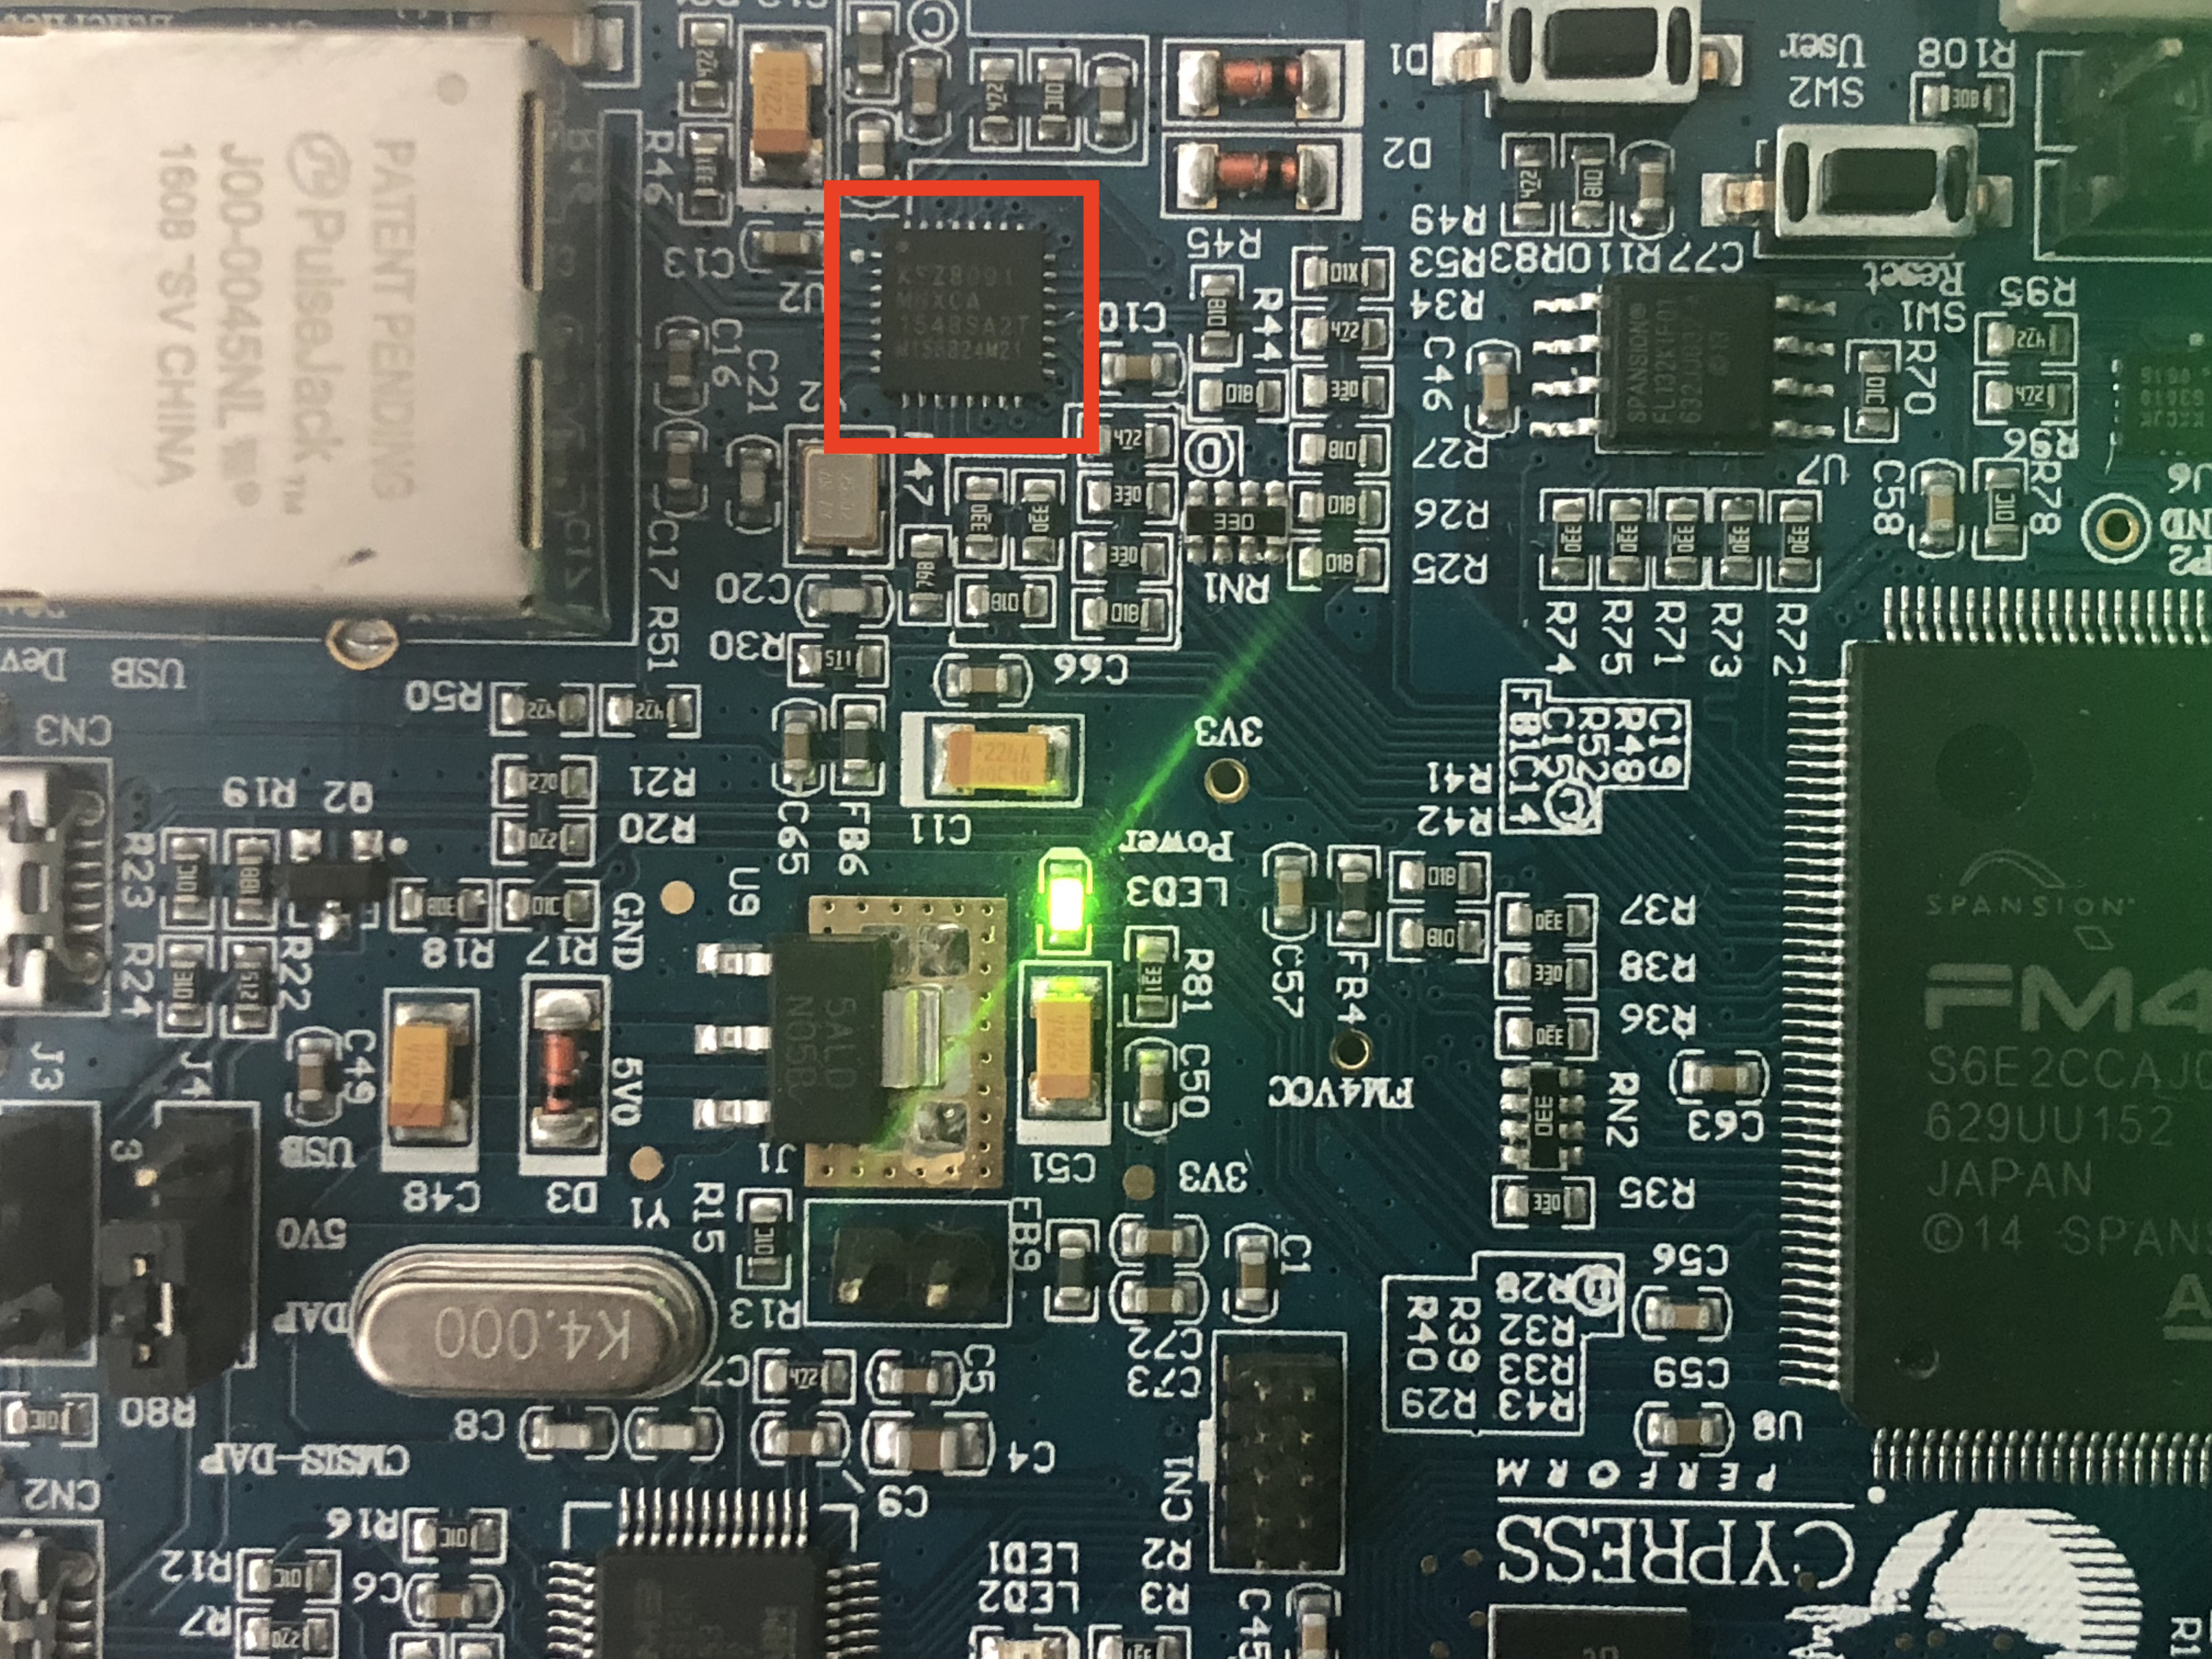
\includegraphics[width=0.4\textwidth]{./05_c/figures/kxcjk1013.jpg}
	\caption{Der Beschleunigungssensor des FM4-Boards}
	\label{fig:accelerometer}
\end{figure} 

In der Datei \lstinline|acceleration.c| findest du eine Vorlage für die Umsetzung einer Wasserwaage mithilfe des Beschleunigungssensors. In dieser fehlt noch die fertige Implementierung der Funktion \lstinline|cppp_rgbLEDAcceleration|. Bei der Initialisierung des Boards wird eine Interrupt-Routine gestartet, sobald neue Messdaten des Beschleunigungssensor des Chips vorliegen. Sofern die Routine ausgelöst wurde, wird \lstinline|cppp_accelerationDataAvailable| auf 1 gesetzt.  
In dem Array \lstinline|float cppp_orientationValues[3]| werden die aktuellen X-,Y- und Z-Achsen-Orientierungen des Boards in alphabetischer Reihenfolge gespeichert. 

\begin{enumerate}
	\item Gebe auf dem Display kontinuierlich die aktuelle Orientierung des Boards aus. Setze hierzu den Cursor per \lstinline|setCursor| an die Position \lstinline|(0,319)| und schreibe die Daten in diesem Format:
%	
	\cpppInputListing{05_c/listings/accelerometerLCDFormat.c}
%	
	\hints{
		\item Verwende zur Ausgabe von Variablen des Typs \lstinline|float| auf den Display die Funktion \lstinline|writeFloat(float value)|.
	}
%
	\item Nutze die Ergebnisse aus Teilaufgabe a) um ein Schema zu Erkennen, wann das Board sich nicht im Gleichgewicht befindet. Setze die RGB-LED auf Rot sofern sich das Board nicht im Gleichgewicht befindet und auf Grün sofern ja. Gebe ebenfalls eine Textausgabe gemäß dem Format oben auf dem Display aus, ob sich das Board im Gleichgewicht befindet. 
	\hints{
		\item Zum Ansteuern der RGB-LED kannst du in dieser Aufgabe als Vereinfachung die Library \lstinline|rgbled.h| verwenden. Hierzu muss zunächst die Funktion \lstinline|cppp_initLEDs| einmalig aufgerufen werden. Mit den Funktionen \lstinline|cppp_red/green/blueLEDOn/Off| kannst du die LEDs an oder ausschalten.
	}
\end{enumerate}


\section{\ExercisePrefixEmbeddedC Android Bluetooth Low Energy \optional}
ABLE (Android Bluetooth Low Energy) ist eine Applikation für Androidgeräte, um über BLE (Bluetooth Low Energy) eine drahtlose Verbindung zwischen einem Android Smartphone und einem anderen beliebigen BLE-Device herzustellen. Der Mikrocontroller des C/C++-Praktikums kann durch ein zusätzliches Modul, welches bereitgestellt wird, mit BLE erweitert werden. Du kannst auf einem Android Smartphone die ABLE Applikation installieren und dich mit dem Mikrocontroller verbinden. Abbildung \ref{fig:ablePreview} zeigt ein Beispielsprogramm indem der Mikrocontroller den X-Wert des Joystick 1 über BLE an ein Android Smartphone sendet. Eine ausführliche Anleitung zur Nutzung von ABLE auf dem Mikrocontroller des Praktikums findest du unter \href{https://github.com/Echtzeitsysteme/able/wiki/Cpp-Lab-Tutorial}{diesem Link [1]}. 
\begin{figure}[!htb]
	\centering
	\includegraphics[width=0.7\textwidth]{./05_c/figures/ABLE_preview.jpg}
	\caption{Der C/C++-Mikrocontroller verbunden über Bluetooth mit einem Android Smartphone}
	\label{fig:ablePreview}
\end{figure} 

% !TeX spellcheck = de_DE
\clearpage

\newboolean{includeWiki}
\setboolean{includeWiki}{false}


\section{\ExercisePrefixEmbeddedC WSN---Wide Sensor Network\optional}
\newcommand{\toolWSN}{\textsc{WSN}\xspace}

\optionaltextboxC

Ein \toolWSN (Wide Sensor Network) ist ein Netzwerk aus verteilten Sensorknoten. Ziel dieser Aufgabe ist es, das Mikrocontrollerboard um weiteren Mikrocontroller mit WiFi-Schnittstelle zu erweitern, sodass mehrere Boards über ein drahtloses Netzwerk (WLAN) kommunizieren können. Dieses Netzwerk soll verwendet werden, um gemessene Sensordaten an eine zentralen Server-Anwendung zu senden.

Als Erweiterungsmodul nutzen wir das ESP-12E Modul. Dieses wird mit einer modifizierten Version der \href{https://github.com/martin-ger/esp_wifi_repeater}{esp\_wifi\_repeater-Firmware} betrieben. Die Kommunikation zwischen unserem Mikrocontroller und dem ESP-Board wird über UART realisiert. 

\begin{enumerate}
	\item Unser Mikrocontrollerboard besitzt insgesamt 12 serielle Schnittstellen. In dieser Aufgabe verwenden wir die Schnittstelle UART3, welche über den Multicon-Pinheader (rote Markierung) verfügbar ist. 
	
	%[Grafiken]
		
	\begin{minipage}{.4\textwidth}
		\centering
		\includegraphics[width=\textwidth]{./05_c/figures/s6e2cc.jpg}
		%\captionof{figure}{Position des Pinheaders auf dem Board}
		%\label{fig:s6e2cc}
	\end{minipage}
	\begin{minipage}{.5\textwidth}		
		\centering
		\includegraphics[width=\textwidth]{./05_c/figures/wsnWiring_Steckplatine.pdf}
		%\captionof{figure}{Verkabelung der Platinen}
		%\label{fig:wiring}
	\end{minipage}

	Zuerst muss das ESP-Board wie in den beiden Abbildungen zu sehen angeschlossen werden. Dazu sind 4 Leitungen nötig: Masse (GND), Versorgungsspannung (Vcc), von Tx (Transmit) am Cypress-Board zu Rx (Receive) am ESP-Modul und vice versa.

	\item Um nun Daten in Form von Zeichenketten zu übertragen, muss zuerst die UART-Schnittstelle initialisiert werden. Dazu reicht es, den Header \lstinline|uart_multicon.h| einzubinden und die Funktion \lstinline|cpp_initUart3Baud(115200)| aufzurufen. \lstinline|115200| ist die Baudrate mit der die Schnittstelle arbeiten muss.
	
	Zum Übertragen von ganzen Zeichenketten, ist es hilfreich zunächst eine Funktion zu implementieren, welche ein einzelnes Zeichen als Parameter entgegennimmt und überträgt (\zB \lstinline|void writeCharUart3(char c)|). In dieser Funktion muss gewartet werden, solange der Aufruf \lstinline|Mfs_Uart_GetStatus(\&UART3, UartTxEmpty)| nicht \lstinline|TRUE| ergibt. \lstinline|TRUE| und \lstinline|FALSE| sind in diesem Fall Makros der Treiberbibliothek, und müssen daher genau so verwendet werden. Liefert der \lstinline|Mfs_Uart_GetStatus|- Aufruf \lstinline|FALSE| zurück, ist die Schnittstelle bereit um ein einzelnes Zeichen mit dem Aufruf von \lstinline|Mfs_Uart_SendData(&UART3, 'c')| zu versenden.
	
	\item Implementiere nun noch eine Funktion die einen nullterminierten C-String entgegennimmt und durch wiederholte Aufrufe von \lstinline|writeCharUart(char c)| versendet.
	
	Teste deine Funktion, indem du ihr einen Text (\zB \lstinline|"mqtt_pub /Hello World!\r\n"|) übergibst. \lstinline|\r\n| markiert das Ende des Befehls. Auf der Serveranwendung sollte deine Nachricht nun ankommen.
	
	\item Erweitere nun dein Board um einen Sensor, und sende den gemessenen Sensorwert an die Zentrale Serveranwendung. Sende dazu den Befehl \lstinline|"mqtt_wsn <Sensorwert>\r\n"|.
\end{enumerate}	

\ifthenelse{\boolean{includeWiki}}{

		\newpage
		\renewcommand{\thesubsection}{}
		\renewcommand{\thesubsubsection}{}
		\subsection{Mini-Wiki}
		
		In diesem Abschnitt sollen die anderen Teile des WSN näher eräutert, und auf deren Funktion eingegangen werden. 
		
		\subsubsection{MQTT} 
		Message Queuing Telemetry Transport (MQTT) ist ein Client-Server-Kommunikationsprotokoll, das auf dem Publish-Subscribe-Muster beruht. Weite Verbreitung hat MQTT in IoT-Szenarien, z.B. bei der Übermittlung von Sensordaten. Ein zentraler Server (Broker) verwaltet hierbei alle Nachrichten in einer hierarchischen Topic-Struktur.  Clients können sich mit dem Broker verbinden und entweder Daten auf einem Topic veröffentlichen (publish), oder ein Topic abonnieren (subscribe), was den Broker dazu veranlasst alle eingehenden Nachrichten eines Topics an den Clienten weiterzuleiten.
			
		Die einzelnen Hierarchiestufen eines Topics werden dabei durch Schrägstriche ('/') voneinander getrennt. Durch Nutzung von Wildcards können nicht nur konkrete Topics, sondern auch Bereiche von Topics abonniert werden. '+' steht dabei als Wildcard für alle Topics der jeweiligen Hierarchiestufe, '\#' schließt auch alle darunterliegenden Topics mit ein, und muss daher immer am Ende der Topic-Definition stehen.
		
		\subsubsection{UART} 
		Universal-Asynchronous-Receiver-Transmitter (UART) ist eine einfache elektronische Schnittstelle zur seriellen Datenübertragung. Es wird häufig verwendet um Daten zwischen Mikrocontrollern und anderen elektronischen Komponenten (e.g. andere Mikrocontroller, Sensoren) auszutauschen.
		
		\subsubsection{WiFi}
		Grundsätzlich gibt es zwei Typen von WiFi-Schnittstellen: Station und Access Point. Eine Station ist in diesem Kontext ein Gerät, welches ein WiFi-Netz aufspannt, eine Station wählt sich in das Netz eines Access-Points ein.
		Die meisten Geräte besitzen nur eine Schnittstelle, und sind somit Station \emph{oder} Access Point.
		
		\subsubsection{ESP12-E}
		Das ESP-12E ist ein Mikrocontrollerboard welches den weit verbreiteten ESP8266 für die Benutzung auf einem Steckbrett optimiert. So stellt es \zB einen Micro-USB Anschluss und zwei Buttons bereit, und führt die Anschlüsse des Mikrocontrollers zum einfacheren Zugriff zu angelöteten Pins.
		
		Im Kontext dieses Projekts ist es wichtig zu erwähnen, dass der ESP8266 in einem kombinierten Modus gleichzeitig als Station und Access Point betrieben werden kann.
		
		\subsubsection{esp\_wifi\_repeater}
		Die esp\_wifi\_repeater-Firmware implementiert die Funktionalität eines NAT-Routers auf dem ESP12E-Board. Da der dort verwendete Mikrocontroller gleichzeitig Station und Access-Point sein kann, ist es möglich ihn als Repeater zu verwenden. Die Firmware bietet im sogenannten \emph{Automesh-Mode} die Möglichkeit der selbstständigen Konfiguration. Im Automesh-Mode werden dem Mikrocontroller nur die SSID und das Passwort des zu Erweiternden Netzwerkes angegeben.
		
		Die Konfigurationsparameter werden dabei auf dem Flashspeicher des Chip geschrieben. Bootet der Chip in diesem Modus, versucht er sich mit einem Netzwerk mit passender SSID zu verbinden. Werden bereits mehrere passende Access Points gefunden, so wählt die Softare stets den Access Point, dessen Signal am stärksten empfangen wird. Gelingt die Verbindung, aktiviert der Mikrocontroller seinen eigenen Access-Point, und erstellt ein eigenes Netzwerk mit derselben Konfiguration, wie das bereits existierende Netzwerk. Das ESP-Board dient nun effektiv als Repeater des vorhandenen WiFi-Netzes. 
		
		Da ein einzelner Repeater immer nur Station genau eines anderen Knoten sein kann, sich jedoch bis zu 8 Stations mit seinem eigenen Access-Point verbinden können (eine Limitierung dieser relativ einfachen Hardware), entsteht so eine Baumtopologie. 
			
		Die Firmware nutzt optional MQTT, um Statusinformationen an einen Broker zu übermitteln.
			
		Im Betrieb kann mit der Firmware in einer Art Kommandozeile über die UART-Schnittstelle des ESP interagiert werden. Die Grundversion stellt zahlreiche Konfigurationsbefehle zur Verfügung. Für diese Aufgabe, wurden zwei neue Kommandos hinzugefügt, die es ermöglichen eigene Daten über den MQTT-Client der Repeater-Software zu senden:
			
			\begin{itemize}		
				\item \lstinline|mqtt_pub <topic> <payload>| veröffentlicht ASCII-Daten (\lstinline|<payload>|) auf dem zu spezifizierenden Topic \lstinline|<topic>|
				
				\item \lstinline|mqtt_wsn <payload>| veröffentlicht ASCII-Daten (\lstinline|<payload>|) auf dem Topic "/WiFi/ESP\_ID/wsn". Darauf veröffentlichte Daten werden von der Desktop-App dem Knoten zugeordnet, und in der Netzwerk-Visualisierung als Sensorwert angezeigt. Es ist daher Sinnvoll eine Einheit mitzusenden, da die Daten sonst jeglichen Kontext verlieren.
			\end{itemize}	
		
		\subsubsection{Desktop-App} 
			Die Desktop-App ist eine Java-Anwendung, deren Aufgabe es ist die aktuelle Netzwerktopologie des Sensornetzwerks zu visualisieren, und übermittelte Sensordaten anzuzeigen. 
			
			Dazu empfängt und verarbeitet sie die von den einzelnen Netzwerkknoten gesendeten Topology-Messages. Die so gewonnenen Informationen ermöglichen es die einzelnen Netzwerkknoten in einer Baumstruktur zusammenzufügen und zu visualisieren. 
			
			Die App implementiert dazu einen MQTT-Clienten, verbindet diesen mit dem Broker, und lässt ihn das Topic \texttt{/WiFi/\#} abonnieren. Topologie-Informationen veröffentlicht jeder Knoten auf einem eigenen Topic "\texttt{/Wifi/ESP\_ID/Topology}", abhängig von seiner ID. Die veröffentlichten Topology-Messages beinhalten im JSON-Format gespeichert unter anderem die MAC-Adresse der AP-Schnittstelle sowie die MAC-Adressen der Stations. Aus den gesendeten MAC-Adressen der Nachbarn, kann so die Baumstruktur gebildet werden. 
	}{}
		


\cclicense

\end{document}
